\documentclass[11pt]{article}
\usepackage[utf8]{inputenc}
\usepackage[T1]{fontenc}
\usepackage{geometry}
\usepackage{hyperref}
\usepackage{enumitem}
\usepackage{tikz}
\usetikzlibrary{positioning}

\geometry{margin=1in}

\title{BS Portfolio 01 MealPlanner}
\author{
  \textit{[Author Name 1]} (\textit{[Matriculation Number]})\\
  \textit{[Author Name 2]} (\textit{[Matriculation Number]})
}
\date{October 27, 2025}

\begin{document}

\maketitle

\section{Project Overview}

\textbf{The Problem.} Food prices for similar products vary dramatically – often by several multiples. Even when comparing different foods based on their nutritional value (proteins, carbohydrates, fats), there are huge price differences per unit of nutrition. This makes it difficult for consumers to make informed decisions about which foods best fit their goals and budget.

\textbf{Our Solution.} The MealPlanner backend allows users to register food items with their prices and nutritional values. The system can then filter and sort these foods by various criteria such as:
\begin{itemize}[noitemsep]
  \item Price per 100g protein
  \item Price per 1000 calories
  \item Protein content per 100g
  \item And many other nutritional and cost metrics
\end{itemize}


This helps users make better decisions about which foods fit their personal goals while achieving them cost-effectively.

\textbf{Dish Management.} Users can also create dishes by adding multiple DishIngredients and filter them using advanced criteria tailored to specific fitness goals:

\begin{itemize}[noitemsep]
  \item \textbf{Protein per serving} – for muscle building priorities
  \item \textbf{Calories per serving} – for general energy management
  \item \textbf{Percentage of calories from protein} – ideal for users combining weight loss with muscle maintenance, as protein slows digestion and increases satiety
  \item \textbf{Caloric density} – enables searching for low-calorie but high-volume meals (perfect for weight loss)
\end{itemize}

This goal-oriented filtering helps users find dishes that match their specific objectives: weight loss users can search for calorie-light but filling meals, muscle building users can prioritize protein-rich dishes, and users with combined goals can focus on high-protein percentage meals for optimal satiety and muscle support.

Once users find a suitable dish, they can automatically add all ingredients to their shopping cart for convenient purchasing. Dishes can also include preparation descriptions and time requirements, with filtering options by preparation time.

\textbf{What We Built.} Our system manages four main components: food items, dishes, users, and shopping carts. Users can create and search through food and dish databases, while the system automatically calculates nutritional values and costs. Everything is measured in grams to keep things simple and consistent. The backend provides fast, filtered search results that help users quickly find what they need.

\textbf{Scope Limitations.} The first increment explicitly excludes allergen/micronutrient modeling and differentiation between coach/client roles – all users have the same capabilities to create food items and dishes as well as filter and purchase them. Unit differentiation (pieces, liters vs. grams) is also excluded to keep the deliverable focused.

\section{Domain Model}

The core entities and relationships appear in Figure~\ref{fig:uml}. The domain layer ensures each dish retains at least one ingredient line, and every line records the gram quantity that drives cost and macronutrient calculations. The model also includes shopping carts that aggregate required grams per \texttt{FoodItem} for purchasing.

\begin{figure}[h]
  \centering
  \resizebox{0.9\linewidth}{!}{%
  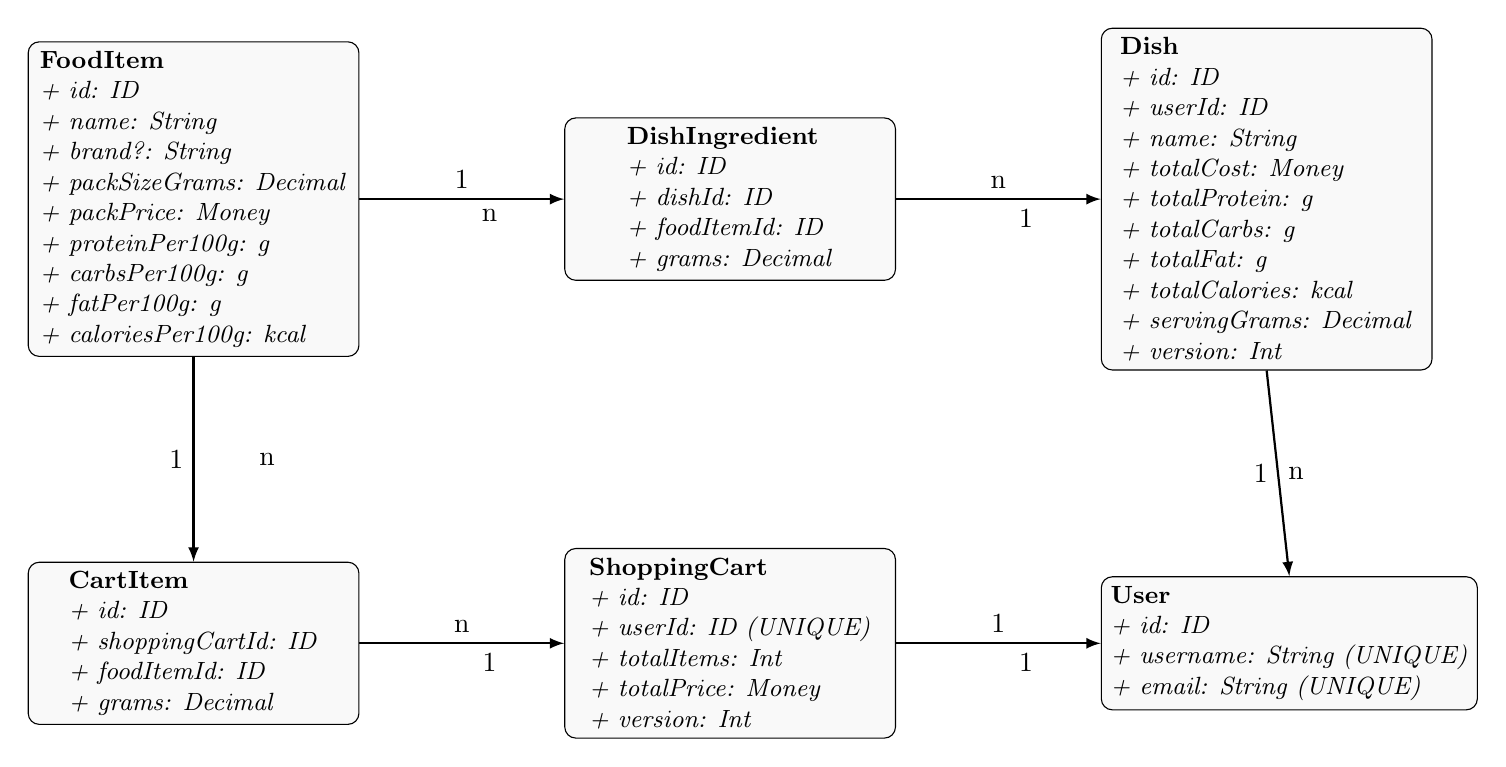
\begin{tikzpicture}[
    class/.style={rectangle, draw, rounded corners, minimum width=4.2cm, align=left, font=\small, fill=gray!5},
    relation/.style={-latex, thick},
    node distance=2.6cm
  ]

    % Row 1: FoodItem, DishIngredient, Dish
    \node[class] (food) {
      \textbf{FoodItem}\\
      \textit{+ id: ID}\\
      \textit{+ name: String}\\
      \textit{+ brand?: String}\\
      \textit{+ packSizeGrams: Decimal}\\
      \textit{+ packPrice: Money}\\
      \textit{+ proteinPer100g: g}\\
      \textit{+ carbsPer100g: g}\\
      \textit{+ fatPer100g: g}\\
      \textit{+ caloriesPer100g: kcal}
    };

    \node[class, right=of food] (dishIng) {
      \textbf{DishIngredient}\\
      \textit{+ id: ID}\\
      \textit{+ dishId: ID}\\
      \textit{+ foodItemId: ID}\\
      \textit{+ grams: Decimal}
    };

    \node[class, right=of dishIng] (dish) {
      \textbf{Dish}\\
      \textit{+ id: ID}\\
      \textit{+ userId: ID}\\
      \textit{+ name: String}\\
      \textit{+ totalCost: Money}\\
      \textit{+ totalProtein: g}\\
      \textit{+ totalCarbs: g}\\
      \textit{+ totalFat: g}\\
      \textit{+ totalCalories: kcal}\\
      \textit{+ servingGrams: Decimal}\\
      \textit{+ version: Int}
    };

    % Row 2: CartItem, ShoppingCart, User
    \node[class, below=of food] (cartItem) {
      \textbf{CartItem}\\
      \textit{+ id: ID}\\
      \textit{+ shoppingCartId: ID}\\
      \textit{+ foodItemId: ID}\\
      \textit{+ grams: Decimal}
    };

    \node[class, right=of cartItem] (cart) {
      \textbf{ShoppingCart}\\
      \textit{+ id: ID}\\
      \textit{+ userId: ID (UNIQUE)}\\
      \textit{+ totalItems: Int}\\
      \textit{+ totalPrice: Money}\\
      \textit{+ version: Int}
    };

    \node[class, right=of cart] (user) {
      \textbf{User}\\
      \textit{+ id: ID}\\
      \textit{+ username: String (UNIQUE)}\\
      \textit{+ email: String (UNIQUE)}
    };

    % Relations
    \draw[relation] (food) -- node[above]{1} node[below]{\quad\quad n} (dishIng);
    \draw[relation] (dishIng) -- node[above]{n} node[below]{\quad\quad 1} (dish);

    \draw[relation] (food) -- node[left]{1} node[right]{\quad\quad n} (cartItem);
    \draw[relation] (cartItem) -- node[above]{n} node[below]{\quad\quad 1} (cart);
    \draw[relation] (cart) -- node[above]{1} node[below]{\quad\quad 1} (user);
    % Vertical from dish bottom to user's top (north)
    \draw[relation] (dish.south) -- node[right]{n} node[left]{1} (user.north);
  \end{tikzpicture}%
  }
  \caption{UML class diagram of the Meal Planner domain.}
  \label{fig:uml}
\end{figure}

\paragraph{Key entities.} \textbf{FoodItem} stores pack size and price plus nutrition per 100\,g (brand is optional). \textbf{DishIngredient} records the grams of a referenced \texttt{FoodItem}. \textbf{Dish} aggregates ingredients and persists total cost and macronutrients together with \textit{servingGrams} and a \textit{version} for optimistic locking. \textbf{ShoppingCart} groups intended purchases per user. \textbf{CartItem} accumulates grams per \texttt{FoodItem}; packs and cost are estimated at query time using \texttt{packSizeGrams} and \texttt{packPrice}. \textbf{User} owns at most one active cart.

\paragraph{Domain invariants.}
\begin{itemize}[noitemsep]
  \item Pack price and size are positive; macro values per 100\,g stay within sensible ranges.
  \item \texttt{DishIngredient.grams} and \texttt{CartItem.grams} are strictly positive.
  \item A \texttt{FoodItem} appears at most once per dish and at most once per cart; adding again merges grams.
  \item Aggregated dish totals (cost and macronutrients) are recomputed transactionally and stored with \texttt{servingGrams}.
  \item Writes to \texttt{Dish} and \texttt{ShoppingCart} use optimistic locking via a \texttt{version} field.
\end{itemize}

\paragraph{Example records.}
\begin{itemize}[noitemsep]
  \item FoodItem: \emph{``Chicken Breast''}, pack size 1{,}000\,g, pack price 7{,}50\,€, protein 23\,g/100\,g, carbohydrates 0\,g/100\,g, fat 1{,}5\,g/100\,g, calories 110\,kcal/100\,g.
  \item Dish: \emph{``Budget Protein Bowl''} with 150\,g Chicken Breast, 100\,g Rice, and 50\,g Broccoli, yielding a total cost of 2{,}45\,€, 38\,g protein, 58\,g carbohydrates, 11\,g fat, and 510\,kcal.
\end{itemize}

\section{Use Cases}

The backend covers six core use cases. Each use case follows a clear structure with preconditions, a main flow, alternate/failure flows, postconditions, and acceptance criteria.

\subsection*{UC01 -- Register Food Item (Must)}
\textbf{Primary Actor:} User\\
\textbf{Goal (User Story):} ``As a user, I want to register an ingredient with correct nutrition and pricing so later calculations are reliable.''\\
\textbf{Preconditions:} The name is unique; pack size and price are positive; macro values per 100\,g are within sensible ranges; brand is optional.\\
\textbf{Main Success Scenario:}
\begin{enumerate}[label=\arabic*.]
  \item The actor submits \texttt{POST /food-items} with name, optional brand, pack size (g), pack price, and protein/carbs/fat/calories per 100\,g.
  \item The service validates values, rounds to two decimals, and computes helper metrics (e.g., price per 100\,g).
  \item The database stores the \texttt{FoodItem} with timestamps.
  \item The API returns \texttt{201 Created} with the id and the saved record.
\end{enumerate}
\textbf{Alternate / Failure Flows:}
\begin{enumerate}[label=\arabic*F.]
  \item Duplicate name $\rightarrow$ \texttt{409 Conflict} with instructions to choose a distinct name.
  \item Out-of-range or negative values $\rightarrow$ \texttt{400 Bad Request} with details.
\end{enumerate}
\textbf{Postconditions:} The \texttt{FoodItem} is stored in a standard format and can be used to compose dishes.\\
\textbf{Acceptance Criteria:}
\begin{itemize}[noitemsep]
  \item Numeric fields are stored with two decimals; invalid values are rejected with clear messages.
  \item Derived metrics (e.g., price per 100\,g) are correct to two decimals.
\end{itemize}

\subsection*{UC02 -- Compose Dish (Must)}
\textbf{Primary Actor:} Nutrition planner\\
\textbf{Goal (User Story):} ``As a planner, I want to create a dish from precise ingredient weights so totals are computed automatically.''\\
\textbf{Preconditions:} At least one \texttt{FoodItem} exists; each ingredient grams value is > 0; each \texttt{FoodItem} appears at most once in the dish.\\
\textbf{Main Success Scenario:}
\begin{enumerate}[label=\arabic*.]
  \item The actor calls \texttt{POST /dishes} with name, servings, and an ingredients array of \{\texttt{foodItemId}, \texttt{grams}\}.
  \item The application service loads the referenced \texttt{FoodItem}s and computes total cost and macronutrients; per-serving values use \texttt{servingGrams}.
  \item The transaction persists \texttt{Dish} and \texttt{DishIngredient} entities atomically.
  \item The API returns \texttt{201 Created} with computed totals and a version number for concurrency.
\end{enumerate}
\textbf{Alternate / Failure Flows:}
\begin{enumerate}[label=\arabic*F.]
  \item Unknown \texttt{foodItemId} $\rightarrow$ \texttt{404 Not Found}.
  \item Duplicate \texttt{foodItemId} in the payload $\rightarrow$ \texttt{400 Bad Request} with guidance to merge grams.
  \item Ingredient grams $\leq 0$ $\rightarrow$ \texttt{400 Bad Request} with validation details.
\end{enumerate}
\textbf{Postconditions:} The dish is stored with correct totals and can be listed and adjusted.\\
\textbf{Acceptance Criteria:}
\begin{itemize}[noitemsep]
  \item Calculated totals equal the sum of ingredient contributions within rounding tolerance.
  \item Saved and fetched representations match, including totals and per-serving values.
\end{itemize}

\subsection*{UC03 -- Adjust Dish Composition (Should)}
\textbf{Primary Actor:} Nutrition planner\\
\textbf{Goal (User Story):} ``As a planner, I want to adjust ingredient weights so that cost and nutrition metrics remain accurate over time.''\\
\textbf{Preconditions:} The dish exists and currently references at least one ingredient.\\
\textbf{Main Success Scenario:}
\begin{enumerate}[label=\arabic*.]
  \item The actor uses sub-resources to modify composition:
    \begin{itemize}[noitemsep]
      \item Add: \texttt{POST /dishes/\{dishId\}/ingredients} with \{\texttt{foodItemId}, \texttt{grams}\}.
      \item Update: \texttt{PATCH /dishes/\{dishId\}/ingredients/\{dishIngredientId\}} with \{\texttt{grams}\}.
      \item Remove: \texttt{DELETE /dishes/\{dishId\}/ingredients/\{dishIngredientId\}}.
    \end{itemize}
  \item The domain validates all changes and recomputes totals, per-serving metrics, and derived rankings.
  \item The persistence layer commits in a single transaction and updates timestamps.
  \item The API returns the refreshed \texttt{Dish} with an incremented version.
\end{enumerate}
\textbf{Alternate / Failure Flows:}
\begin{enumerate}[label=\arabic*F.]
  \item Concurrent modification $\rightarrow$ \texttt{409 Conflict} with retry guidance.
  \item Removing all ingredients $\rightarrow$ \texttt{400 Bad Request} with ``Dish must contain at least one ingredient.''
\end{enumerate}
\textbf{Postconditions:} The dish reflects updated totals and remains consistent for listing and ranking.\\
\textbf{Acceptance Criteria:}
\begin{itemize}[noitemsep]
  \item Per-serving calculations update consistently after each modification.
  \item Versioning prevents overwrites and clearly signals conflicts.
\end{itemize}

\subsection*{UC04 -- Add Dish to Shopping Cart (Should)}
\textbf{Primary Actor:} Shopper preparing groceries\\
\textbf{Goal (User Story):} ``As a shopper, I want to add a whole dish to my shopping cart so that all its ingredients are added in the correct quantities automatically.''\\
\textbf{Preconditions:} The target \texttt{Dish} exists; an active shopping cart exists (or is created implicitly); \texttt{servingsMultiplier} is a positive integer.\\
\textbf{Main Success Scenario:}
\begin{enumerate}[label=\arabic*.]
  \item The actor calls \texttt{POST /shopping-carts/\{cartId\}/items/from-dish} with \{\texttt{dishId}, optional \texttt{servingsMultiplier}=1\}.
  \item The application service loads the dish and its \texttt{DishIngredient}s.
  \item For each ingredient, the service creates or increments a \texttt{CartItem} for the \texttt{foodItemId} with grams = \texttt{ingredient.grams} \(\times\) \texttt{servingsMultiplier}.
  \item The transaction persists all item changes and returns the updated cart state.
\end{enumerate}
\textbf{Alternate / Failure Flows:}
\begin{enumerate}[label=\arabic*F.]
  \item Unknown \texttt{dishId} or \texttt{cartId} $\rightarrow$ \texttt{404 Not Found}.
  \item Non-positive \texttt{servingsMultiplier} $\rightarrow$ \texttt{400 Bad Request} with validation details.
  \item Concurrent write to the same cart $\rightarrow$ \texttt{409 Conflict}; ask the user to retry.
\end{enumerate}
\textbf{Postconditions:} The shopping cart contains one item per \texttt{FoodItem} in the dish; grams are merged into existing items instead of duplicating lines.\\
\textbf{Acceptance Criteria:}
\begin{itemize}[noitemsep]
  \item Adding a dish creates or increments per-\texttt{FoodItem} items by \(\texttt{ingredient.grams} \times \texttt{servingsMultiplier}\).
  \item Re-adding the same dish with \texttt{servings = n} increases the same items cumulatively; no duplicate rows are created.
  \item When two dishes share a \texttt{FoodItem}, the cart reflects the summed grams across both additions.
\end{itemize}

\subsection*{UC05 -- Filter and Rank Food Items (Must)}
\textbf{Primary Actor:} Shopper or nutrition planner\\
\textbf{Goal (User Story):} ``As a user, I want to search, filter, and sort food items by cost and nutrition so that I can identify the best options for my goals and budget.''\\
\textbf{Preconditions:} At least one \texttt{FoodItem} exists with valid derived metrics.\\
\textbf{Main Success Scenario:}
\begin{enumerate}[label=\arabic*.]
  \item The actor calls \texttt{GET /food-items} with query parameters for filtering (e.g., min/max protein per 100\,g) and sorting (e.g., price per 100\,g protein).
  \item The application service builds a database query that uses derived metrics consistently.
  \item The API returns a paginated list including the requested sort order and summary fields.
\end{enumerate}
\textbf{Alternate / Failure Flows:}
\begin{enumerate}[label=\arabic*F.]
  \item No matching items $\rightarrow$ \texttt{200 OK} with an empty array.
  \item Unsupported filter or sort parameter $\rightarrow$ \texttt{400 Bad Request} listing allowed fields and formats.
\end{enumerate}
\textbf{Postconditions:} The actor receives a consistently ordered list of food items aligned to their constraints.\\
\textbf{Acceptance Criteria:}
\begin{itemize}[noitemsep]
  \item Sorting by price-per-protein and other metrics is stable and repeatable.
  \item Pagination metadata and caching headers are present and correct.
\end{itemize}

\subsection*{UC06 -- Cart Summary and Pack Estimates (Should)}
\textbf{Primary Actor:} Shopper preparing purchases\\
\textbf{Goal (User Story):} ``As a shopper, I want a consolidated shopping cart summary with estimated packs and total cost so that I can purchase the right amounts efficiently.''\\
\textbf{Preconditions:} The shopping cart exists and contains one or more items; each referenced \texttt{FoodItem} has a known pack size and pack price.\\
\textbf{Main Success Scenario:}
\begin{enumerate}[label=\arabic*.]
  \item The actor calls \texttt{GET /shopping-carts/\{cartId\}/summary}.
  \item The service sums grams per \texttt{FoodItem} across all cart items.
  \item For each \texttt{FoodItem}, the service computes \textit{estimatedPacks} = \(\lceil\,\texttt{totalGrams} / \texttt{packSizeGrams}\,\rceil\) and \textit{estimatedCost} = \(\texttt{estimatedPacks} \times \texttt{packPrice}\).
  \item The API returns the consolidated list with totals for cost and macronutrients.
\end{enumerate}
\textbf{Alternate / Failure Flows:}
\begin{enumerate}[label=\arabic*F.]
  \item Unknown \texttt{cartId} $\rightarrow$ \texttt{404 Not Found}.
  \item Missing pack size or price for a referenced item $\rightarrow$ \texttt{422 Unprocessable Entity} with guidance on how to fix.
\end{enumerate}
\textbf{Postconditions:} The actor receives a clear summary that can be used for purchasing and budgeting.\\
\textbf{Acceptance Criteria:}
\begin{itemize}[noitemsep]
  \item Estimated packs are rounded up correctly; cost totals equal the sum of per-item estimates.
  \item Macro totals across the cart equal the sum of all items within rounding.
\end{itemize}

\end{document}
